\documentclass[11pt, twocolumn]{article}
\usepackage{titlesec}
\usepackage{tikz}
\usepackage{booktabs}
\usepackage{adjustbox} 
\usepackage{enumitem}
\usepackage{multirow}
\usepackage{bbding,enumitem}
\usepackage{authblk}
\usepackage{fancyhdr}
\usepackage{amsmath}
\usepackage{subcaption}
\usepackage[table]{xcolor}
\setcounter{secnumdepth}{3} % for adjusting padding
\pagestyle{fancy}
\newcommand{\blueoval}{%
    \begin{tikzpicture}[remember picture, overlay]
    \shade[shading=axis, left color=blue, right color=white] (current page.north west) -- (3,0) arc (0:180:4cm) -- cycle;
    \end{tikzpicture}%
}

\newcommand{\coloredfooter}{%
    \begin{tikzpicture}[remember picture, overlay]
    \shade[shading=axis, left color=teal, right color=white] (current page.south east) -- (-1,-2) arc (0:80:2cm) -- cycle;
    \end{tikzpicture}%
}

\fancyhf{} % Clear default header and footer
\fancyhead[L]{ \leftmark}
% Display section title in the left header
\fancyhead[R]{\thepage} % Display page number in the right header
\definecolor{mypink3}{cmyk}{0, 0.7808, 0.4429, 0.1412}

\makeatletter
\renewcommand{\maketitle}{\bgroup\setlength{\parindent}{0pt}
\begin{flushleft}
  \textbf{\@title}

  \@author
\end{flushleft}\egroup
}
\makeatother

\title{\Huge \color{mypink3}{ROV Document}  \vspace{0.5cm}}
\author{\Large E-JUST Robotics Club \normalsize \hspace{0.5cm} }

\setlength{\parindent}{0pt}
\date{\today}

\usepackage[showframe=false, margin=.75in]{geometry}

\usepackage{abstract}
\renewcommand{\abstractname}{}    % clear the title
\renewcommand{\absnamepos}{empty} % originally center

\usepackage{lipsum}

\usepackage{afterpage}

\renewenvironment{abstract}
 {\small
  \begin{center}
  \bfseries \abstractname\vspace{-.5em}\vspace{0pt}
  \end{center}
  \list{}{%
    \setlength{\leftmargin}{10mm}% <---------- Change margin here
    \setlength{\rightmargin}{\leftmargin}%
  }%
  \item\relax}
 {\endlist}

\usepackage[utf8]{inputenc}

%\usepackage{graphicx}
\usepackage{wrapfig}
\usepackage[lofdepth,lotdepth]{subfig}
\usepackage{booktabs}

\usepackage{rotating}

\usepackage{caption}
%\usepackage{subcaption}

%\usepackage[ngerman]{babel}

\usepackage{csquotes}

\setlength{\marginparwidth}{2cm} % Set marginparwidth to avoid todonotes issues
\usepackage{todonotes}

\usepackage{stfloats}

\usepackage[T1]{fontenc}
\usepackage{textcomp}
\usepackage{times}

\usepackage{framed} %um Boxen zu machen

\usepackage[citestyle=authoryear,
			bibstyle=authoryear,
			language=auto,
			url=false,
			backend=bibtex,
			doi=false,
			isbn=false]{biblatex}
	\renewbibmacro*{volume+number+eid}{%
  \printfield{volume}%
%  \setunit*{\adddot}% DELETED
  \setunit*{\addnbspace}% NEW (optional); there's also \addnbthinspace
  \printfield{number}%
  \setunit{\addcomma\space}%
  \printfield{eid}}
\DeclareFieldFormat[article]{number}{\mkbibparens{#1}}

\usepackage{setspace}
\onehalfspacing

\setlength{\columnsep}{0.8cm}

\setlength{\parskip}{0em}

\usepackage{color}
\definecolor{black}{gray}{0} % 10% gray

\usepackage[colorlinks=true,linkcolor=black,citecolor=black]{hyperref}

\usepackage{tabularx}
\newcolumntype{s}{>{\hsize=.5\hsize}X}

\usepackage{ntheorem}
\newtheorem*{TRQ}{Research Question}

\newtheorem{Hyp}{Hypothesis} 

\usepackage{graphicx}
\usepackage{fancyhdr}
\usepackage{lipsum}
\usepackage{geometry}
\usepackage{changepage} % To adjust page margins locally
\usepackage{afterpage}

% Apply the custom header and footer to all pages
\fancyfoot[L]{\hspace*{-1.9cm}{\includegraphics[width=\paperwidth,height=1.9cm]{Images/Footer.png}}} % Footer

\pagestyle{fancy}
\makeatletter
\providecommand{\sf@counterlist}{} % Define sf@counterlist to avoid undefined control sequence
\makeatother

\usepackage{titlesec}

\titlespacing*{\subsection}{0pt}{5pt}{5pt}
\titlespacing*{\subsubsection}{0pt}{5pt}{5pt}

\setcounter{secnumdepth}{4}
\renewcommand\theparagraph{\thesubsubsection.\arabic{paragraph}}

\usepackage{tabularray}
\DefTblrTemplate{firsthead,middlehead,lasthead}{default}{}
\DefTblrTemplate{firstfoot}{default}{
  \UseTblrTemplate{contfoot}{default}
  \UseTblrTemplate{caption}{default}
}
\DefTblrTemplate{middlefoot}{default}{
  \UseTblrTemplate{contfoot}{default}
  \UseTblrTemplate{capcont}{default}
}
\DefTblrTemplate{lastfoot}{default}{
  \UseTblrTemplate{note}{default}
  \UseTblrTemplate{remark}{default}
  \UseTblrTemplate{capcont}{default}
}
\DefTblrTemplate{contfoot-text}{default}{Continue on the next column}
\DefTblrTemplate{capcont}{default}{\UseTblrTemplate{caption}{default}}
\UseTblrLibrary{booktabs}
\captionsetup{skip=3pt}
\SetTblrInner{rowsep=0pt, stretch=0.9}
\setlength{\headheight}{13.6pt}
\addtolength{\topmargin}{-1.6pt}
\setlength{\footskip}{58.2pt}

\begin{document}
\onecolumn

\tableofcontents
\clearpage

\twocolumn

\section{Mechanical Safety Features}

\subsection{Canister}

\begin{itemize}[leftmargin=0pt, itemindent=10pt]
    \setlength{\itemsep}{0pt}
    \item The electronic casings of ROVs are securely sealed with an IP rating (IP68), ensuring protection against dust particles and the ability to endure pressures at depths of up to 5 meters underwater.
    
    \begin{figure}[h!]
        \centering
        \includegraphics[width=\columnwidth]{Images/kamikaze.jpeg}
        \caption{Kamikaze.}
        \label{fig:kamikaze}
    \end{figure}

    \item The clamp strain relief (Figure \ref{fig:strain}) secures the wires to prevent disconnecting from the canister, ensuring the integrity and reliability of the ROV’s electrical system. Metal glands—positioned at the base of the canister—are sized to match the wire diameters, creating a tight seal around the opening and effectively preventing water ingress.
    
    \begin{figure}[h!]
        \centering
        \includegraphics[width=\columnwidth]{Images/strain releif.jpeg}
        \caption{Strain relief and Sleeved tether.}
        \label{fig:strain}
    \end{figure}
\break
    \item For Sealing enhancement:
    \vspace{-0.3cm}
    \begin{itemize}
        \setlength{\itemsep}{0pt}
        \item Sikadur-31 CF adhesive prevents micro-gaps and enhances waterproofing.
        \item IP68-rated metallic cable glands ensure watertight cable entry points while maintaining flexibility. 
        \item Epoxy resin and super glue reinforce adhesion between PETG and aluminum, eliminating potential leaks.
        \item Bolted mechanical fastening provides long-term stability and prevents structural deformation.
    \end{itemize}
    
\end{itemize}

\subsection{Thrusters}

\begin{itemize}[leftmargin=0pt, itemindent=10pt]
    \setlength{\itemsep}{0pt}
    \item The thruster assemblies feature specialized protective structures designed to minimize the possibility of foreign objects being drawn in. These guards incorporate mesh elements of suitable size in accordance with IP 20 ingress protection standards (Figure \ref{fig:thruster}). Such setup effectively prevents external objects from interfering with the thruster blades.
    
    \begin{figure}[h]
        \centering
        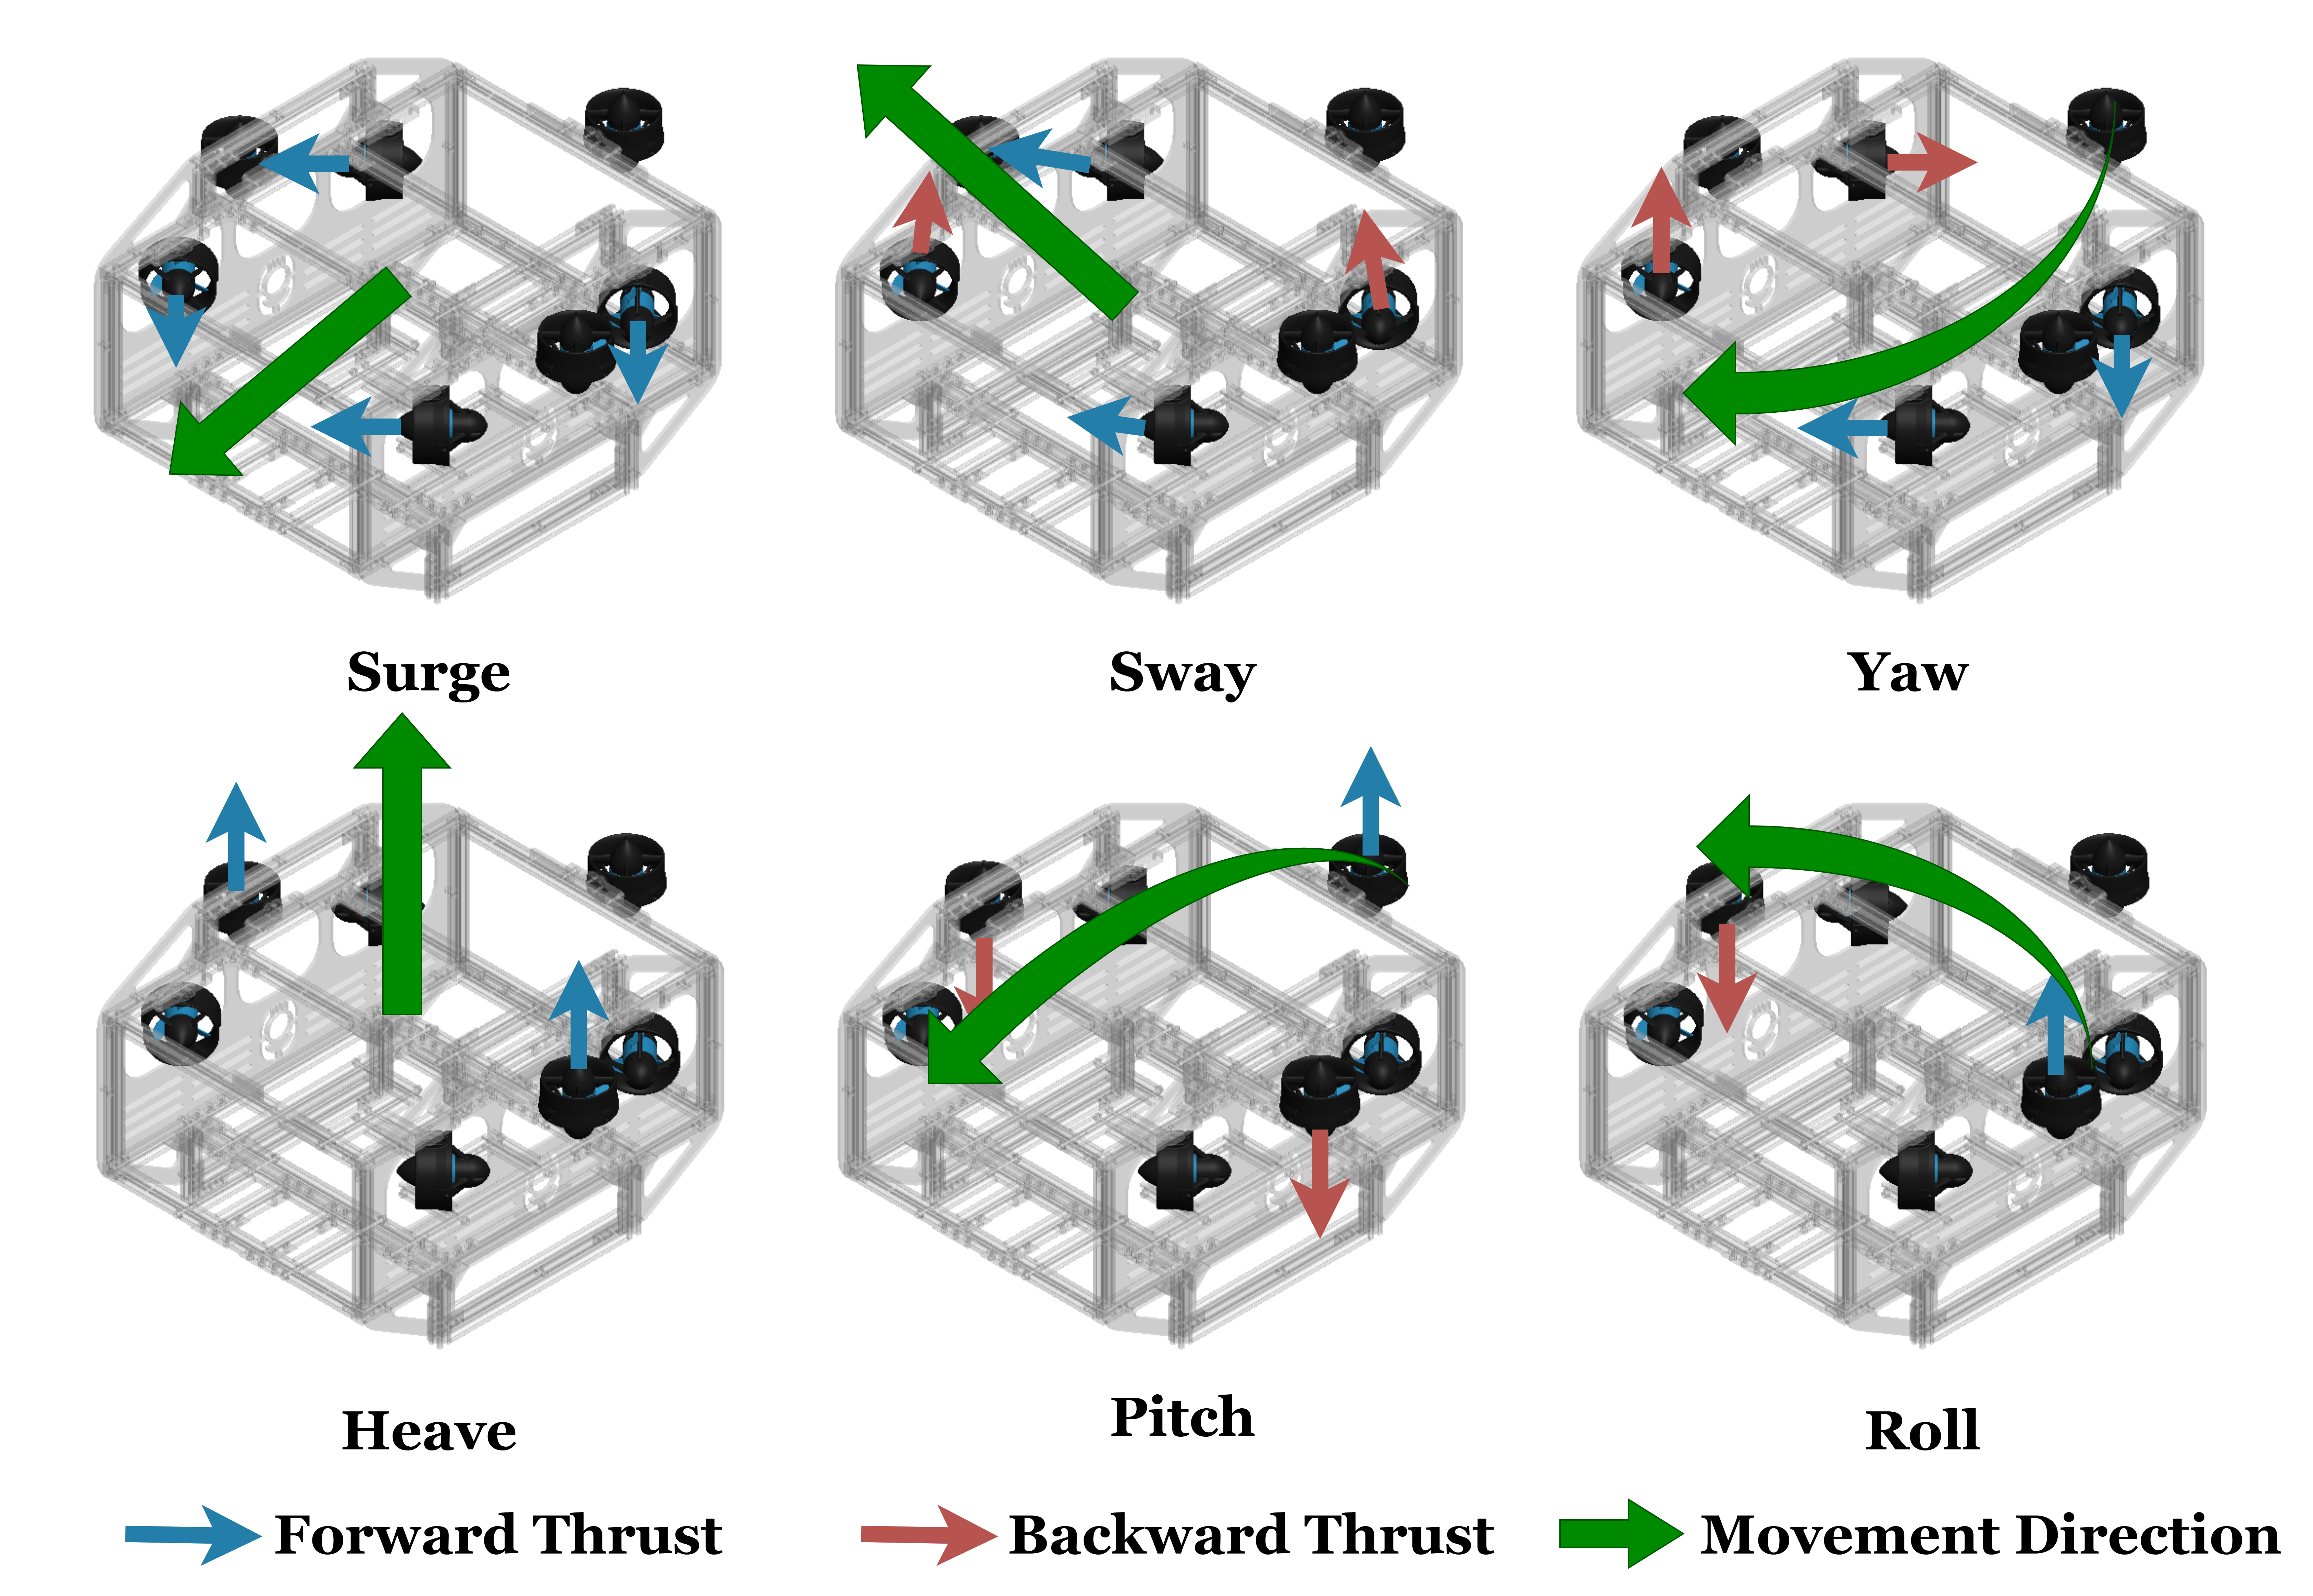
\includegraphics[width=0.6\columnwidth]{Images/Thrusters.jpeg}
        \caption{Shrouded Thrusters.}
        \label{fig:shrouds}
    \end{figure}

    \item The ROV employs a smooth exterior design, eliminating sharp corners and edges. This design approach minimizes the potential for snagging or entanglement with personnel or environmental features, enhancing operational safety.
\end{itemize}

\section{Pneumatic Safety Features}

\subsection{Fluid power quiz}

As the company considered using pneumatic power, we have taken and passed the online fluid power quiz with a score of 100\%. As a result, we were listed among the passing teams on the official website of MATE ROV as shown below in Figure \ref{fig:quiz}.

\begin{figure}[ht!]
    \centering
    \includegraphics[width=\columnwidth]{Images/QUIZ (1).png}
    \caption{Fluid Power Quiz Screenshot.}
    \label{fig:quiz}
\end{figure}

\subsection{Pressure}

\begin{itemize}[leftmargin=0pt, itemindent=10pt]
    \setlength{\itemsep}{0pt}
    \item The air compressor shows no signs of external rust, and the wiring is properly secured (Figure \ref{fig:compressor}). It is equipped with a pressure relief valve (Figure \ref{fig:releif_valve}) installed before the pressure regulator. The regulator is set to 0.275 MPa (Figure \ref{fig:regulator}), equivalent to 40 psi, which complies with the maximum allowable pressure specification.
    \item To comply with the specified maximum allowable pressure of 40 psi (0.275 MPa or 2.75 bar) for pneumatic systems, it is essential that the components used have a minimum pressure rating of 100 psi (0.69 MPa or 6.9 bar)
    \item We did not utilize either a pressurized cylinder or pressure storage device that would need to comply with the MATE specifications.

    \begin{figure}[h] 
        \centering
        \begin{subfigure}[b]{0.49\columnwidth} 
            \centering
            \includegraphics[width=\linewidth]{Images/Air Compressor.jpg}
            \caption{Air Compressor.}
            \label{fig:compressor}
        \end{subfigure}
        \hfill
        \begin{subfigure}[b]{0.49\columnwidth}
            \centering
            \includegraphics[width=\linewidth]{Images/Pressure Relief Valve.jpg}
            \caption{Pressure Relief Valve.}
            \label{fig:releif_valve}
        \end{subfigure}
    
        \vspace{0.2cm}
    
        \begin{subfigure}[b]{0.49\columnwidth}
            \centering
            \includegraphics[width=\linewidth]{Images/Pressure Regulator.jpg}
            \caption{Pressure Regulator.}
            \label{fig:regulator}
        \end{subfigure}
        \hfill
        \begin{subfigure}[b]{0.49\columnwidth}
            \centering
            \includegraphics[width=\linewidth]{Images/Air Service Unit.jpg} 
            \caption{Air Service Unit.}
            \label{fig:air_service_unit}
        \end{subfigure}
    
        \caption{Pneumatic Components.}
        \label{fig:pneumatic_components}
    
    \end{figure}
\end{itemize}

\subsection{Pressure ratings}

Listed below are the pressure ratings of the pneumatic components that were used.

\begin{itemize}[leftmargin=0pt, itemindent=10pt]
    \setlength{\itemsep}{0pt}
    \vspace{-0.3cm}
    \item \textbf{Air Service Unit:} As shown in (Figure \ref{fig:air_service_unit}), the maximum rated pressure for the unit is 9.9 kgf/cm² which is equivalent to 140 psi.
    \item \textbf{Solenoid Directional Control Valve:} The valve's maximum pressure is rated as 0.8 MPa which surpasses the minimum pressure specified, as shown in Figure \ref{fig:solenoid}.
    \begin{figure}[h!]
        \centering
        \includegraphics[width=0.6\columnwidth]{Images/Solenoid Directional Control.jpg}
        \caption{Solenoid Directional Control.}
        \label{fig:solenoid}
    \end{figure}
    \vspace{-0.3cm}
    \item \textbf{Fittings:} The pressure of all pneumatic fittings is rated to 1 MPa or above which makes them comply with the minimum pressure rating.
    \item \textbf{Pneumatic Hose:} The working pressure of the hose is rated at 10 bars, exceeding the minimum pressure specified. 
    \item \textbf{Non-return Valve:} The pressure rating of the non-return valve is 0.8 MPa so it meets the specification of the minimum pressure rating.
\end{itemize}

\vspace{-0.3cm}
\subsection{Fluid SID}

Our Fluid SID is shown in Figure \ref{fig:fluid_sid}.
\vspace{-0.3cm}
\begin{figure}[h!]
    \centering
    \includegraphics[width=\columnwidth]{Images/Pneumatic SID.jpg}
    \caption{Fluid SID.}
    \label{fig:fluid_sid}
\end{figure}

\vspace{-1cm}
\section{Electrical Safety Features}
\vspace{-0.3cm}
\subsection{Anderson Power pole}

Anderson Power pole connectors are the main point of connection in the ROV, known for their ease of use and reliability. They can reduce the risk of damage and electrical hazards during assembly, disassembly, maintenance, or repair work. The connectors are color-coded to prevent incorrect connections and reduce the risk of electrical shorts or other issues, especially in the limited visibility of the underwater environment.

\begin{table*}[b]
    \centering
    \begin{adjustbox}{max width=0.95\textwidth}
    \begin{tabular}{@{} l *{5}{c} @{}}
      \toprule
      \textbf{Component} & \textbf{Quantity} & \textbf{Voltage (V)} & \textbf{Current (A)} & \textbf{Power Per Unit (W)} & \textbf{Total Power (W)} \\
      \midrule
      T200 Thruster            & 7 & 12   & 12     & 144    & 1008   \\
      Basic ESC                & 7 & 12   & 0.15   & 1.8    & 12.6   \\
      Raspberry Pi 5           & 1 & 5    & 5      & 25     & 25     \\
      STM32                    & 4 & 3.3  & 0.125  & 0.4125 & 1.65   \\
      MCP2515 CAN Bus Module   & 5 & 5    & 0.1    & 0.5    & 2.5    \\
      W5500 Ethernet Module    & 1 & 5    & 0.13   & 0.65   & 0.65   \\
      Arduino Nano RP2040      & 1 & 5    & 0.45   & 2.25   & 2.25   \\
      720p USB Camera          & 3 & 5    & 0.2    & 1      & 3      \\
      1080p USB camera         & 2 & 5    & 0.275  & 1.375  & 2.75   \\
      MS5837 Depth Sensor      & 1 & 5    & 0.002  & 0.01   & 0.01   \\
      ZED 2i stereo camera     & 1 & 5    & 0.5    & 2.5    & 2.5    \\
      \midrule
     \multicolumn{5}{l}{\textbf{Total}} & \textbf{1060.91} \\
      \bottomrule
    \end{tabular}
    \end{adjustbox}
\caption{Power Calculation for the ROV.}
\label{tab:rov_power_calculation}
\end{table*}

\subsection{Control Box}

\begin{itemize}[leftmargin=0pt, itemindent=10pt]
    \setlength{\itemsep}{0pt}
    \item For the control box, AC wiring is not used, there is no exposed wiring, and all components inside the canister are insulated with heat wrap to protect against any potential leakage.
    
    \item Used a laptop and Joystick for controlling. (Figure \ref{fig:station})
    
    \begin{figure}[h!]
        \centering
        \includegraphics[width=0.8\columnwidth]{Images/Station.png}
        \caption{Topside Control Station.}
        \label{fig:station}
    \end{figure}
\end{itemize}

\vspace{-0.3cm}
\subsection{Fuse Calculations}
\subsubsection{ROV Side}

As shown in Table \ref{tab:rov_power_calculation} is the calculations of the ROV side. Total Current Drawn = 1060.9/48 = 21.10 A

Total Current Drawn at 48V: \( 1060.9 / 48 = 21.10 \, \text{A} \), Applying Safety Factor: \( 1.3 \times 21.10 = 28.73 \, \text{A} \)
\setlength{\parskip}{0pt}

Required Fuse = 30A

\subsubsection{Non-ROV Side}

As shown in Table 2 is the calculations of the Non- ROV side.

\begin{table}[h!]
  \centering
  \begin{adjustbox}{max width=\columnwidth}
  \begin{tabular}{@{} l *{5}{c} @{}}
    \toprule
    \textbf{Component} & \textbf{Quantity} & \textbf{Voltage (V)} & \textbf{Current (A)} & \textbf{Power Per Unit (W)} & \textbf{Total Power (W)} \\
    \midrule
    NRF24L01            & 1 & 3.3   & 0.115     & 0.3795    & 0.3795   \\
    RTC Module                & 1 & 5   & 0.1   & 0.5    & 0.5   \\
    EEPROM           & 1 & 5    & 0.01      & 0.05     & 0.05     \\
    STM32 F411           & 1 & 5   & 0.25      & 0.25     & 0.25   \\
    Pumps/Motors	& 2	& 12	& 1	& 12	& 24 \\
    \midrule
   \multicolumn{5}{l}{\textbf{Total}} & \textbf{26.1795} \\
    \bottomrule
  \end{tabular}
  \end{adjustbox}
\caption{Power Calculation for the Non-ROV Device.}
\label{tab:power_calculation}
\end{table}

Total Power = 26.18W

Safety Factor = 1.5

Result = 3.2724375

Required Fuse: 5A

\subsection{Low-level Fuses}

\begin{itemize}[leftmargin=0pt, itemindent=10pt]
    \setlength{\itemsep}{0pt}

    \item A 15A fuse is placed on each thruster to ensure that the thrusters do not consume more power than planned, preventing any potential damage to the DC-DC converters.
    \item A properly sized little fuse is within 30 cm of the main point of connection to 48- volt power. (Figure \ref{fig:fuse})
    
    \begin{figure}[h!]
        \centering
        \includegraphics[width=0.8\columnwidth]{Images/fuse.png}
        \caption{Sized Little Fuse.}
        \label{fig:fuse}
    \end{figure}
\end{itemize}

\begin{figure*}[hb!]
    \centering
    \includegraphics[width=\textwidth]{Images/electrical SID.png}
    \caption{Electrical SID.}
    \label{fig:electrical_sid}
\end{figure*}

\subsection{Tether}

Proper wire connection to the tether and the ROV through strain relief is essential to ensure the safety and reliability of the ROV’s electrical components. To achieve this, all tether wires are enclosed in a protective sleeve, with additional strain relief mechanisms, such as cable ties or other fasteners, to keep them secure and prevent damage during operation.

\subsection{Isolation and Marking}

All components will be safely isolated inside the canister, which will be marked along with the thrusters and any exposed working mechanisms to ensure they do not pose any risk to viewers. Additionally, all components inside the canister are insulated with heat wrap to protect against any potential leakage.

\subsection{Electrical SID}

Electrical SID is shown in Figure \ref{fig:electrical_sid}.

\end{document}
